\documentclass{beamer}
\usepackage[utf8]{inputenc}
\usepackage[english]{babel}

% -- Including some standard packages --
\usepackage{graphicx}
\usepackage{soul}
\usepackage{hyperref}
\usepackage{colortbl}
\usepackage{dsfont}
\usepackage{soul}

% -- Choosing theme --

\usetheme{Boadilla}
\usecolortheme{whale}
\setbeamercolor{alerted text}{fg=purple} % Making alerted text non-red

% Tikz
\usepackage{tikz}
\usetikzlibrary{matrix,positioning,fit,backgrounds,intersections}

% -- Cross signs --
\usepackage{pifont} % http://ctan.org/pkg/pifont
\newcommand{\cmark}{\ding{51}}%
\newcommand{\xmark}{\ding{55}}%
\newcommand{\xopt}{\ding{48}}%

% -- Custom commands --
\DeclareMathOperator*{\argmax}{arg\,max}
\DeclareMathOperator*{\argmin}{arg\,min}

\title[Mathematics I]{\textbf{Mathematics for Cryptographers. Preliminaries.}}
\author{ZKDL Camp}
\date{July 18, 2024}
\titlegraphic{
    
\includegraphics[width=0.2\textwidth]{images/logo.png}
}

\expandafter\def\expandafter\insertshorttitle\expandafter{%
  \insertshorttitle\hfill%
  \insertframenumber\,/\,\inserttotalframenumber}

\AtBeginSection[]{
  \begin{frame}
  \vfill
  \centering
  \begin{beamercolorbox}[sep=8pt,center,shadow=true,rounded=true]{title}
    \usebeamerfont{title}\insertsectionhead\par%
  \end{beamercolorbox}
  \vfill
  \end{frame}
}

\begin{document}
    \frame {
      \titlepage
    }
  
    \begin{frame}{Plan}
      \tableofcontents
    \end{frame}

    \section{Some words about the course}
    \begin{frame}{About ZKDL} 

      \begin{itemize}
        \item ZKDL Camp is a series of lectures and workshops on zero-knowledge proofs and cryptography.
        \item Here, we will learn state-of-the-art zero-knowledge systems: what are SNARKs, how they work under the hood from total scratch.
        \item If possible, we will conduct workshops, where we will show practical implementations of the theoretical material.
        \item Primary audience: cryptographers, R\&D Engineers, ZK developers, and everyone wanting to boost their understanding of cryptography.
      \end{itemize}

      \begin{alertblock}{Note}
        This is not a regular course: we require a lot of commitment and the material is fairly complex. However, we will try to make it as simple as possible.
      \end{alertblock}

    \end{frame}

    \begin{frame}{Approximate Camp Structure}
      \begin{enumerate}
        \item Mathematics Preliminaries (3-4 lectures): group and number theory, finite fields, polynomials, elliptic curves etc.
        \item Deep Delve into SNARKs: General definition, arithmetic circuits, commitment schemes, encryption etc.
        \item Analysis of modern zero-knowledge proving systems: Groth16, Plonk, BulletProofs, STARK etc.
        \item Specialization topics: low-level optimizations, advanced protocols such as folding schemes, Nova etc.
      \end{enumerate}
    \end{frame}

    \section{Notation}

    \subsection{Sets}

    \begin{frame}{Sets}
      \begin{definition}
        \textbf{Set} is a collection of distinct objects, considered as an object in its own right.
      \end{definition}

      \begin{example}
        \begin{itemize}
          \item $\mathbb{N}$ is a set of natural numbers.
          \item $\mathbb{Z}$ is a set of integers.
          \item $\mathbb{R}$ is a set of real numbers.
          \item $\mathbb{C}$ is a set of complex numbers.
          \item $\{1, 2, 5, 10\}$ is a set of four elements.
          \item $\{1, 2, 2, 3\}$ simply equals to $\{1,2,3\}$ -- we do not count duplicates.
        \end{itemize}
      \end{example}
    \end{frame}

    \begin{frame}{Operations on sets}
    % --- Writing diagrams ---
    \def\firstcircle{(0,0) circle (1.5cm)}
    \def\secondcircle{(0:2cm) circle (1.5cm)}

    \colorlet{circle edge}{blue!50}
    \colorlet{circle area}{blue!20}

    \tikzset{filled/.style={fill=circle area, draw=circle edge, ultra thick},
        outline/.style={draw=circle edge, ultra thick}}    

      \begin{figure}
        \begin{center}
        \begin{tabular}{cc}
        % Set A and B
        \begin{tikzpicture}
            \begin{scope}
                \clip \firstcircle;
                \fill[filled] \secondcircle;
            \end{scope}
            \draw[outline] \firstcircle node {$A$};
            \draw[outline] \secondcircle node {$B$};
            \node[anchor=south] at (current bounding box.north) {$A \cap B$};
        \end{tikzpicture} &   
        %Set A or B but not (A and B) also known a A xor B
        \begin{tikzpicture}
            \draw[filled, even odd rule] \firstcircle node {$A$}
                                        \secondcircle node{$B$};
            \node[anchor=south] at (current bounding box.north) {$\overline{A \cap B}$};
        \end{tikzpicture}
        \\
        % Set A or B
        \begin{tikzpicture}
            \draw[filled] \firstcircle node {$A$}
                        \secondcircle node {$B$};
            \node[anchor=south] at (current bounding box.north) {$A \cup B$};
        \end{tikzpicture} &  
        % Set A but not B
        \begin{tikzpicture}
            \begin{scope}
                \clip \firstcircle;
                \draw[filled, even odd rule] \firstcircle node {$A$}
                                            \secondcircle;
            \end{scope}
            \draw[outline] \firstcircle
                        \secondcircle node {$B$};
            \node[anchor=south] at (current bounding box.north) {$A \setminus B$};
        \end{tikzpicture}
    \end{tabular}
    \end{center}
    \label{fig:venn_diagrams}
    \end{figure}
    \end{frame}
    
    \begin{frame}{Defining sets}
      \begin{example}
        \begin{itemize}
          \item $\{x \in \mathbb{R}: x^2 = 1\}$ -- a set of real numbers that satisfy the equation $x^2 = 1$.
          \item $\{x \in \mathbb{Z}: x \text{ is even}\}$ -- a set of even integers.
          \item $\{x^2: x \in \mathbb{R}, x^3 = 1\}$ -- a set of squares of real numbers that satisfy the equation $x^3 = 1$.
          \item $\{x \in \mathbb{N}: x \text{ is prime}\}$ -- a set of prime natural numbers.
        \end{itemize}
      \end{example}

      \begin{alertblock}{Question \#1}
        How to simplify the set $\{x \in \mathbb{N}: x^2 = 2\}$?
      \end{alertblock}
  
      \begin{alertblock}{Question \#2(*)}
        How to simplify the set $\{\sin \pi k: k \in \mathbb{Z}\}$?
      \end{alertblock}
    \end{frame}

    \subsection{Logic}
    \begin{frame}{Basic Logic}
        \begin{itemize}
          \item $\forall$ means ``for all''.
          \item $\exists$ means ``there exists''.
          \item $\land$ means ``and''.
          \item $\lor$ means ``or''.
        \end{itemize}

        \begin{alertblock}{Question \#1}
            Is it true that $(\forall x \in \mathbb{N}): \{x > 0\}$?
        \end{alertblock}

        \begin{alertblock}{Question \#2}
            Is it true that $(\exists x \in \mathbb{N}): \{x \geq 0 \land x < 1\}$?
        \end{alertblock}

        \begin{alertblock}{Question \#3}
            Is it true that $(\forall x \in \mathbb{Z})\, (\exists y \in \mathbb{N}): \{y > x\}$?
        \end{alertblock}
    \end{frame}

    \subsection{Randomness and Sequences}

    \begin{frame}{Randomness and Sequences}
        \begin{block}{Notation}
          To denote probability of event $E$, we use notation $\text{Pr}[E]$. For example,
          \begin{equation*}
              \text{Pr}[\text{It will be cold tomorrow}] = 0
          \end{equation*}
        \end{block}

        \begin{block}{Notation}
            To denote that we take an element from a set $S$ uniformly at random, we use notation $x \xleftarrow{R} S$.

            For example, when throwing a coin, we can write $x \xleftarrow{R} \{\text{heads}, \text{tails}\}$.
        \end{block}

        \begin{block}{Notation}
          To denote an infinite sequence $x_1,x_2,\cdots$, we use $\{x_i\}_{i \in \mathbb{N}}$. To denote
          a finite sequence $x_1,x_2,\cdots,x_n$, we use $\{x_i\}_{i=1}^n$. To enumerate 
          through a list of indeces $\mathcal{I} \subset \mathbb{N}$, we use notation
          $\{x_i\}_{i \in \mathcal{I}}$.
        \end{block}
    \end{frame}

    \section{Basic Group Theory}

    \subsection{Reasoning behind Groups}
    \begin{frame}{Why Groups?!}
        Well, first of all, we want to work with integers\ldots

        Imagine that Alice pays to Bob with a card number $N$, but instead of paying to a number $N$, the system pays 
        to another card number $N+k, k \ll N$, which is only by 0.001\% different. Bob would not be 99.999\% happy\ldots

        \begin{figure}
          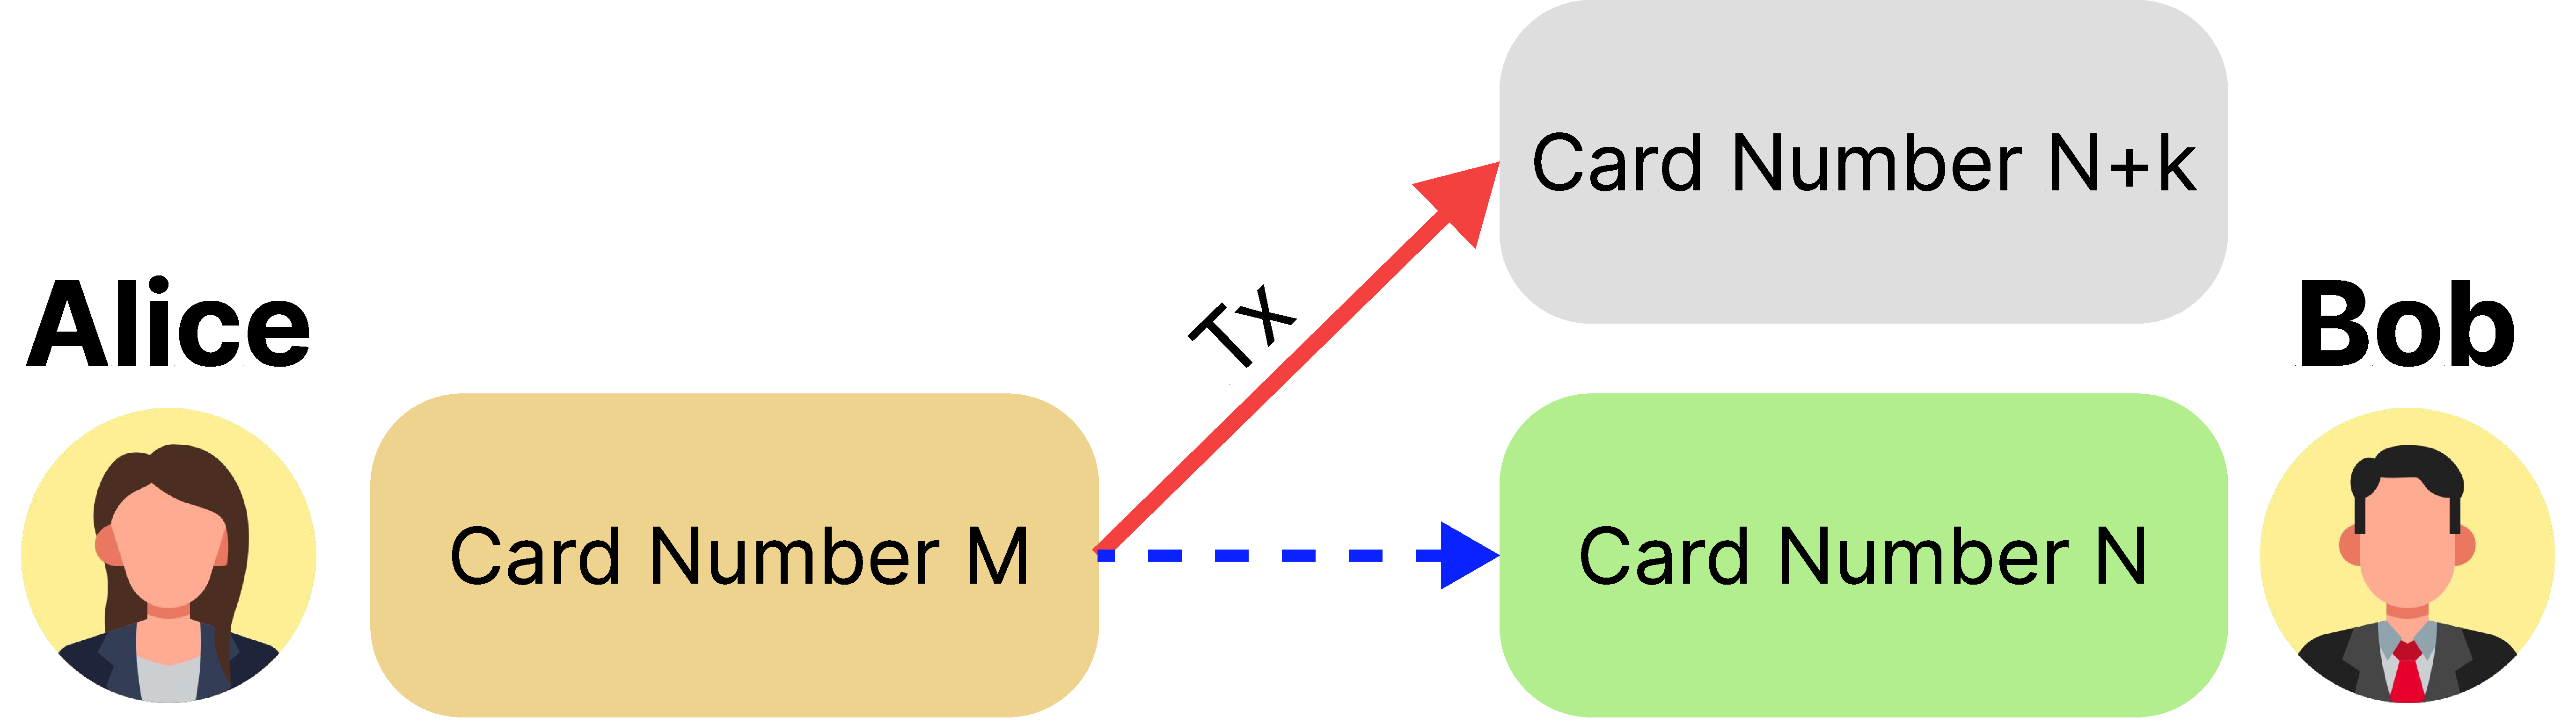
\includegraphics[width=1.0\textwidth]{images/lecture_1/why_integers.pdf}
          \label{fig:why_integers}
        \end{figure}
    \end{frame}

    \begin{frame}{Why Groups?!}
        But integers on their own are not enough. We need to define a structure that allows us to perform operations on them.

        This is very similar to interfaces: we abstract from the implementation, just merely stating we have ``some'' addition/multiplication.

        \begin{example}
            Consider set $\mathbb{G} := \{\text{Dmytro}, \text{Dan}, \text{Friendship}\}$. We can safely define an operation $\oplus$ as:
            \begin{gather*}
                \text{Dmytro} \oplus \text{Dan} = \text{Friendship} \\ 
                \text{Dan} \oplus \text{Friendship} = \text{Dmytro} \\
                \text{Friendship} \oplus \text{Dmytro} = \text{Dan}
            \end{gather*}
        \end{example}

        \begin{block}{Rethorical question}
            What makes $(\mathbb{G}, \oplus)$ a group?
        \end{block}
    \end{frame}
    \subsection{Group Definition and Examples}
    \begin{frame}{Group Definition}
      \begin{definition}
        \textbf{Group} $(\mathbb{G}, \oplus)$, is a set with a binary operation $\oplus$ with following rules:
        \begin{enumerate}
            \item \textbf{Closure:} Binary operations always outputs an element from $\mathbb{G}$, that is $\forall a,b \in \mathbb{G}: a \oplus b \in \mathbb{G}$.
            \item \textbf{Associativity:} $\forall a,b,c \in \mathbb{G}: (a \oplus b)\oplus c = a \oplus (b \oplus c)$.
            \item \textbf{Identity element:} There exists a so-called identity element $e \in \mathbb{G}$ such that $\forall a \in \mathbb{G}: e \oplus a = a \oplus e = a$.
            \item \textbf{Inverse element:} $\forall a \in \mathbb{G} \; \exists b \in \mathbb{G}: a\oplus b = b \oplus a = e$. We commonly denote the inverse element as $(\ominus a)$.
        \end{enumerate}
    \end{definition}

    \begin{definition}
        A group is called \textbf{abelian} if it satisfies the additional rule called \textbf{commutativity}: $\forall a,b \in \mathbb{G}: a \oplus b = b \oplus a$.
    \end{definition}
    \end{frame}

    \begin{frame}{Explanation for Developers: Trait}
      \begin{center}
        \begin{figure}
          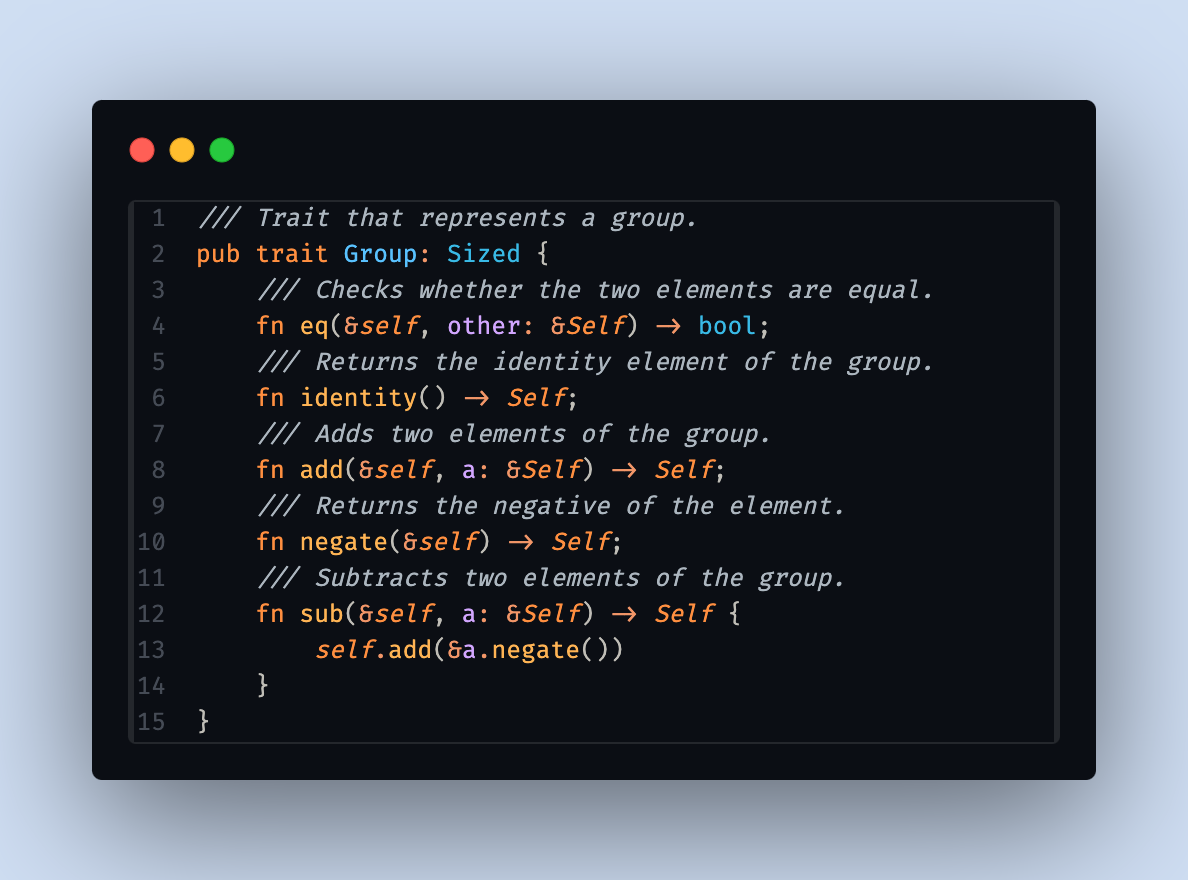
\includegraphics[width=0.8\textwidth]{images/lecture_1/group_in_rust.png}
          \label{fig:group_in_rust}
        \end{figure}

        More on that: \url{https://github.com/ZKDL-Camp/lecture-1-math}.
      \end{center}
    \end{frame}

    \begin{frame}{Group Examples}
      \begin{example}
        A group of integers with the regular addition $(\mathbb{Z},+)$ (also called the \textit{additive} group of integers) is a group.
      \end{example}
      
      \begin{example}
          The multiplicative group of positive real numbers $(\mathbb{R}_{> 0}, \times)$ is a group for similar reasons. 
      \end{example}
      
      \begin{alertblock}{Question \#1}
          Is $(\mathbb{R}, \times)$ a group? If no, what is missing?
      \end{alertblock}

      \begin{alertblock}{Question \#2}
        Is $(\mathbb{Z}, \times)$ a group? If no, what is missing?
      \end{alertblock}
    \end{frame}

    \begin{frame}{Small Note on Notation}
      \begin{block}{Additive group}
          We say that a group is \textit{additive} if the operation is denoted as $+$, and the identity element is denoted as $0$.
      \end{block}

      \begin{block}{Multiplicative group}
          We say that a group is \textit{multiplicative} if the operation is denoted as $\times$, and the identity element is denoted as $1$.
      \end{block}
      \begin{block}{Rule of thumb}
        We use additive notation when we imply that the group $\mathbb{G}$ is the set of points on the elliptic curve, while multiplicative is typically used in the rest of the cases.
      \end{block}
  \end{frame}

    \begin{frame}{Abelian Groups Examples and Non-Examples}
      \begin{alertblock}{Question \#3}
        Is $(\mathbb{R}, -)$ a group? If no, what is missing?
      \end{alertblock}
      \begin{alertblock}{Question \#4}
          Set $V$ is a set of tuples $(v_1,v_2,v_3)$ where each $v_i \in \mathbb{R} \setminus \{0\}$. Define the operation $\odot$ as
          \begin{equation*}
              (v_1,v_2,v_3) \odot (u_1,u_2,u_3) = (v_1u_1, v_2u_2, v_3u_3)
          \end{equation*}

          Is $(V, \odot)$ a group? If no, what is missing?
      \end{alertblock}
      \begin{block}{Conclusion}
        Group is just a fancy name for a set with a binary operation that behaves nicely.
      \end{block}
    \end{frame}

    \subsection{Subgroup}
    \begin{frame}{Subgroup}

      \begin{alertblock}{Question}
          Suppose $(\mathbb{G}, \oplus)$ is a group. Is any subset $\mathbb{H} \subset \mathbb{G}$ a group?
      \end{alertblock}

      \begin{definition}
          A \textbf{subgroup} is a subset $\mathbb{H} \subset \mathbb{G}$ that is a group with the same operation $\oplus$. We denote it as $\mathbb{H} \leq \mathbb{G}$.
      \end{definition}

      \begin{example}
          Consider $(\mathbb{Z}, +)$. Then, although $\mathbb{N} \subset \mathbb{Z}$, it is not a subgroup, as it does not have inverses.
      \end{example}

      \begin{example}
          Consider $(\mathbb{Z}, +)$. Then, $3\mathbb{Z} = \{3k: k \in \mathbb{Z}\} \subset \mathbb{Z}$ is a subgroup.
      \end{example}
  \end{frame}

  \begin{frame}{Tiny question}
    \begin{alertblock}{Question}
      Does any group have at least one subgroup?
  \end{alertblock}

  Yeah, $\mathbb{H} = \{e_{\mathbb{G}}\} \leq \mathbb{G}$.
  \end{frame}

  \subsection{Homomorphism and Isomorphism}

  \begin{frame}{Homomorphism}
    \begin{definition}
      A \textbf{homomorphism} is a function $\phi: \mathbb{G} \rightarrow \mathbb{H}$ between two groups $(\mathbb{G}, \oplus)$ and $(\mathbb{H}, \odot)$ that preserves the group structure, i.e., 
      \begin{equation*}
        \forall a,b \in \mathbb{G}: \phi(a \oplus b) = \phi(a) \odot \phi(b)
      \end{equation*}
    \end{definition}

    \begin{example}
      Consider $(\mathbb{Z}, +)$ and $(\mathbb{R}_{>0}, \times)$. Then, the function $\phi: \mathbb{Z} \rightarrow \mathbb{R}_{>0}$ defined as $\phi(k) = 2^k$ is a homomorphism.
    \end{example}

    \textbf{Proof}. Take any $n,m \in \mathbb{Z}$ and consider $\phi(n+m)$:
    \begin{equation*}
      \phi(n+m) = 2^{n+m} = 2^n \times 2^m = \phi(n) \times \phi(m)
    \end{equation*}
  \end{frame}

  \begin{frame}{Mapping types}
    \begin{figure}
      \includegraphics[width=0.7\textwidth]{images/lecture_1/mapping.pdf}
      \label{fig:mappings}
    \end{figure}
  \end{frame}

  \begin{frame}{Homomorphism}
    \begin{definition}
      \textbf{Isomorphism} is a bijective homomorphism.
    \end{definition}

    \begin{definition}
      Two groups $\mathbb{G}$ and $\mathbb{H}$ are \textbf{isomorphic} if there exists an isomorphism between them. We denote it as $\mathbb{G} \cong \mathbb{H}$.
    \end{definition}

    \begin{example}
     $\phi: k \mapsto 2^k$ from the previous example is a homomorphism between $(\mathbb{Z},+)$ and $(\mathbb{R}_{>0},\times)$, but not an isomorphism. Indeed, there is no $x \in \mathbb{Z}$ such that $2^x = 3 \in \mathbb{R}_{>0}$.
    \end{example}

    \begin{alertblock}{Question}
      What can we do to make $\phi$ an isomorphism?
     \end{alertblock}
  \end{frame}

  \begin{frame}{Field}
    \begin{definition}{}
        \textbf{Field} $K$ is a set equipped with appropriate \textbf{addition} and \textbf{multiplication} operations with the corresponding well-defined inverses, where you can perform the basic arithmetic.
    \end{definition}
    \pause
    \begin{exampleblock}{}
        \begin{itemize}
            \item $\mathbb{R}$ (real numbers) is a field.
            \item $\mathbb{Q}$ (rational numbers) is a field.
            \item $\mathbb{C}$ (complex numbers) is a field.
            \item $\mathbb{N}$ (natural numbers) is not a field: there is no additive inverse for $2$ ($-2$ is not in $\mathbb{N}$).
            \item $\mathbb{Z}$ (integers) is not a field: additive inverse is defined, but the multiplicative is not ($2^{-1}$ is not defined).
        \end{itemize}
    \end{exampleblock}
\end{frame}

    \section{Polynomials}

      
  
    \begin{frame}{}
        \centering \Large
        \emph{Thanks for your attention!}
      \end{frame}
\end{document}